%---------TODO----------
% Crear una figura mejor
% nanotubos de carbono, dinámica molecular ademas (ensamble nose-hoover y parrinello-rahman), LINCS
\chapter{Mecánica Estadística de Equilibrio}
\section{Fundamentos teóricos}
La mecánica estadística estudia propiedades de los sistemas macroscópicos termodinámicos a partir de sus propiedades microscópicas. Una cantidades macroscópica de estado (ó macroestado $(U,V,N)$) en un sistema, es el promedio de propiedades microscópicas. Un estado microscópico del sistema es un punto en el espacio fase $(q,p)$ correspondiente al macroestado $(U,V,N)$ este se conoce como microestado y el total de microestados asociados a un macroestado se denota por $\Omega(U,V,N)$.\\

Sin embargo, resolver la dinámica del sistema por cualquiera de los métodos en dinámica (Newton, Lagrange o Hamilton) seria un cálculo imposible y largo. Dos postulados fundamentales de la física estadística crean dicha conexión entre ambas escalas \cite{tuckerman2010}: \\

\begin{itemize}
    \item Postulado de equiprobabilidad: En un sistema aislado todos sus microestados accesibles son igualmente probables, i.e., a un macroestado de equilibrio le corresponden mayor número de microestados.\\
    
    \item Postulado de la entropía: En un sistema en equilibrio, su entropía esta dada por:
    \begin{equation}
        S=Kln(\Omega)
    \end{equation}
    con K una constante y $\Omega$ el numero de microestados correspondientes.
\end{itemize}


\section{Ensambles}

Un ensamble es un conjunto hipotético de $N$ replicas de un sistema que se encuentra en un macroestado dado y cada replica esta en algún microestado accesible.\\

Los ensambles pueden ser definidos dependiendo de las situaciones termodinámicas que se impongan al sistema, y dependiendo de estos se pueden extraer propiedades estáticas macroscópicas como la energía, temperatura, presión, etc. Los ensambles que cumplen esta propiedad estática aun cuando el sistema se encuentra evolucionando en el tiempo se les llaman: \textit{Ensambles de equilibrio}.\\

En teoría clásica de ensambles todas las observables macroscópicas de un sistema están conectados a una función microscópica. Por el primer postulado, se puede calcular el promedio temporal de una variable dinámica $A$ como en la ecuacion \ref{promediotemp}, o por un promedio de ensamble asociado a su probabilidad \ref{promedioequprob} \cite{tuckerman2010}. \\

\begin{equation} \label{promediotemp}
    \langle A\rangle = \lim_{t\to\infty}\frac{1}{t}\int_0^t A(t)dt
\end{equation}\\

\begin{equation} \label{promedioequprob}
    \langle A\rangle =\sum_r A_r P_r
\end{equation}\\

con $P_r$ la probabilidad del r-ésimo microestado y $A_r$ el valor de $A$ en el r-ésimo microestado.\\

\begin{table}[h!]
    \centering
    \begin{tabular}{ |p{1cm}||p{4cm}|  }
    \hline
    \multicolumn{2}{|c|}{Ensambles} \\
    \hline
    NVE   & Microcanónico \\
    NVT   & Canónico \\
    $\mu$VT& Gran Canónico \\
    NPT   & Isotérmico-Isobárico \\
    \hline
    \end{tabular}
    \caption{Tipos de Ensambles}
    \label{tiposEnsamble}
\end{table}

\subsection{Ensamble Canónico NVT}

Este ensamble esta formado por $\mathcal{N}$ copias de un sistema en equilibrio con una fuente de calor a temperatura T. Imaginemos que los $\mathcal{N}$ sistemas del ensamble están en contacto entre si mediante paredes diatérmicas, i.e., para cada sistema en este ensamble, el resto es su fuente de calor como se muestra en la figura \ref{fig:CanonicEns}.\\

\begin{figure}[!h]
    \centering
    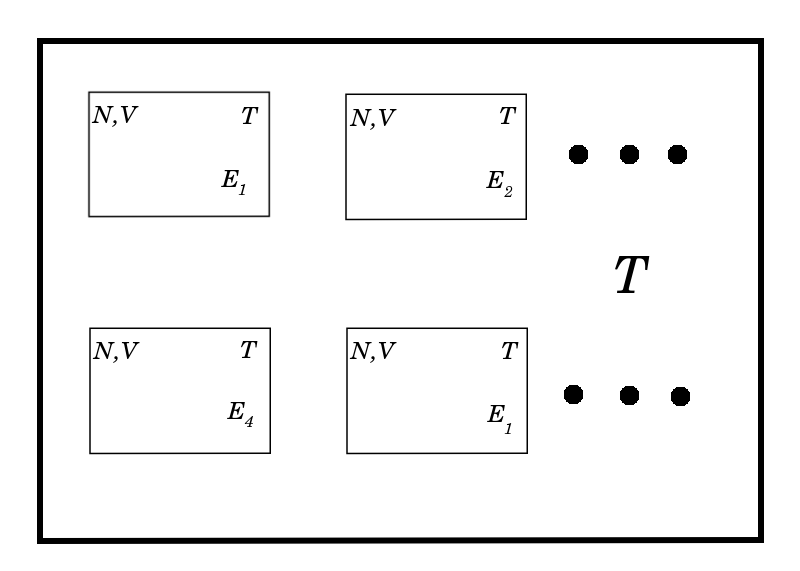
\includegraphics[width=.55\textwidth,keepaspectratio=true]{EnsCanonico.png}
    \caption{Representación del ensamble canónico NVT \cite{belof2013alternative}}
    \label{fig:CanonicEns}
\end{figure}

\newpage

Las partes del ensamble se encuentran en alguno de los $E_r$ niveles de energía, estos a su vez toman y ceden energía con su alrededor, es decir, los otro microestados. Notar que puede haber degeneración de algunos microestados.\\

Tenemos:\\
\begin{center}
    $N_1$ sistemas con energía $E_1$\\
    $N_2$ sistemas con energía $E_2$\\
    ...\\
    $N_r$ sistemas con energía $E_r$\\
    ...\\
\end{center}


Cumple:

\begin{equation} \label{restrprob}
    1 = \sum_r P_r \\
\end{equation}

\begin{equation} \label{energiaprob}
    E = U = \langle E\rangle = \sum_r P_r E_r
\end{equation}

\begin{center}
    con $P_r = \frac{N_r}{\mathcal{N}}$
\end{center}


El número de formas de microestados correspondientes en que se presenta esta distribución es:\\

\begin{equation}
    \Omega = \frac{\mathcal{N}!}{\prod_r N_r}
\end{equation}\\

Y por el postulado de la entropía y de acuerdo a la formula de Stirling:

\begin{equation}  \label{entropiaboltz}
    S = kln(\frac{\mathcal{N}}{\prod_r N_r}) = -K\mathcal{N}\sum_r P_rln(P_r)
\end{equation}\\

Usando el método de los multiplicadores de Lagrange se encuentra la función de partición canónica $\mathcal{Z}$:

\begin{equation} \label{probcan}
    P_r = \frac{e^{-\beta E_r}}{\mathcal{Z}}
\end{equation}
\begin{equation} \label{funcpartcan}
    \mathcal{Z} = \sum_r e^{-\beta E_r \quad con\ \beta=\frac{1}{KT}
\end{equation}

La entropía dentro de unos de los sistemas del ensamble es \cite{mandl1988statistical}:

\begin{equation}
    S = k\beta U + kln(\mathcal{Z})
\end{equation}

Todas las propiedades termodinámicas se obtienen de la función de partición canónica:

\begin{equation} \label{energcan}
    U=-\frac{\partial}{\partial \beta}ln(\mathcal{Z})
\end{equation}

\begin{equation} \label{ecestacan}
    PV=KTln(\mathcal{Z})
\end{equation}

El potencial termodinámico del ensamble canónico es la energía libre de Helmholtz:

\begin{equation} \label{potHelm}
    F(N,V,T)=-\frac{1}{\beta}ln(\mathcal{Z})=U-TS
\end{equation}

\subsection{Ensamble isotérmico-isobárico NPT}

El ensamble NPT esta formado por $\mathcal{N}$ copias de un sistema en equilibrio con una fuente de calor a temperatura T y una fuente de Volumen. Los $\mathcal{N}$ sistemas de este ensamble estan en contacto entre si por paredes diatérmicas y flexibles.\\

\begin{figure}[!h]
    \centering
    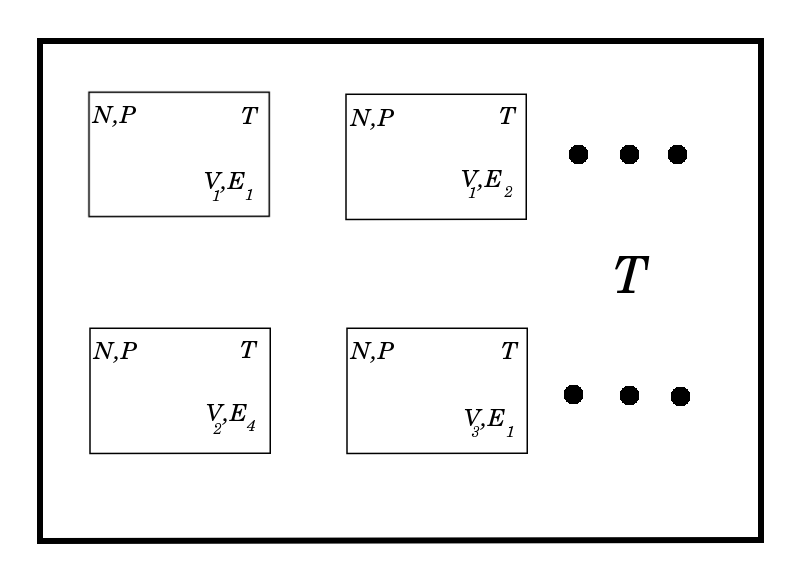
\includegraphics[width=.55\textwidth,keepaspectratio=true]{nptensemble.png}
    \caption{Representación del ensamble NPT \cite{belof2013alternative}}
    \label{fig:NPTEns}
\end{figure}

\newpage

Tenemos en este sistema lo siguiente:\\

\begin{center}
    $N_{1n}$ sistemas con energía $E_{1n}$ y volumen $V_1$\\
    $N_{2n}$ sistemas con energía $E_{2n}$ y volumen $V_2$\\
    ...\\
    $N_{rn}$ sistemas con energía $E_{rn}$ y volumen $V_r$\\
    ...\\
\end{center}

Lo anterior debe cumplir con:

\begin{equation} \label{restrprobNPT}
    1 = \sum_r P_r \\
\end{equation}

\begin{equation} \label{energiaprobNPT}
    U = \langle E\rangle = \sum_{rn} P_{rn} E_{rn}
\end{equation}

\begin{equation} \label{volprobNPT}
    V = \langle E\rangle = \sum_{rn} P_{rn} V_r
\end{equation}

\begin{center}
    con $P_{rn} = \frac{N_{rn}}{\mathcal{N}}$
\end{center}

El número de formas de microestados correspondientes en que se presenta esta distribución es:\\

\begin{equation} \label{distribucionmultnom}
    \Omega = \frac{\mathcal{N}!}{\prod_{rn} N_{rn}}
\end{equation}\\

Y por el postulado de la entropía y de acuerdo a la formula de Stirling:

\begin{equation}  \label{entropiaboltzNPT}
    S = kln(\frac{\mathcal{N}}{\prod_{rn} N_{rn}}) = -K\mathcal{N}\sum_{rn} P_{rn} ln(P_{rn})
\end{equation}\\

Usando el método de los multiplicadores de Lagrange se encuentra la función de partición para el ensamble NPT $\mathcal{Z}$:

\begin{equation} \label{probNPT}
    P_{rn} = \frac{e^{-\beta E_{rn}-\xi V_r}}{\mathcal{Z}}
\end{equation}
\begin{equation} \label{funcpartNPT}
    \mathcal{Z} = \sum_{rn} e^{-\beta E_{rn}-\xi V_r} \quad con\ \beta=\frac{1}{KT} \quad y\ \xi=\frac{P}{KT}
\end{equation}

La entropía de uno de los sistemas del ensamble es \cite{mcquarrie1976}:

\begin{equation}
    S = k\beta U + k\xi V + kln(\mathcal{Z})
\end{equation}

Todas las propiedades termodinámicas se obtienen de la función de partición encontrada:

\begin{equation} \label{energNPT}
    U=-\frac{\partial}{\partial \beta}ln(\mathcal{Z})
\end{equation}

\begin{equation} \label{volNPT}
    V=-\frac{\partial}{\partial \xi}ln(\mathcal{Z})
\end{equation}

\begin{equation} \label{ecestaNPT}
    PV=KTln(\mathcal{Z})
\end{equation}

El potencial termodinámico del ensamble isotérmico-isobárico es la energía libre de Gibbs \cite{mcquarrie1976}:

\begin{equation} \label{potgibbs}
    G(N,P,T)=-\frac{1}{\beta}ln(\mathcal{Z})=U-TS+PV
\end{equation}\\

\section{Mecánica estadística clásica de N partículas interactuantes
}

En las aplicaciones de la mecánica estadística mas comunes están los cálculos que tienen solución exacta, donde las partículas no interactuan en los sistemas. Sin embargo, esto no siempre es posible en sistemas donde las particulas interactuan, por eso es importante

Supongamos un fluido con $\mathcal{N}$ partículas que interactuan a través de un potencial $\mathcal{V}$ y es conservativo. En el formalismo lagrangiano las ecuaciones de movimiento son \cite{torresdelcastillo_2018}:\\

\begin{equation} \label{lagrangeeq}
    \frac{d}{dt}\frac{\partial L}{\partial \dot r_i} - \frac{\partial L}{\partial \dot r_i} = 0
\end{equation}\\

donde $L$ es el lagrangiano del sistema:

\begin{equation} \label{lagrangiano}
    L = \sum_{i=1}^{N} \frac{1}{2}m_i\dot{\vec{r_i}}^2-\mathcal{V}({\vec{r}}_1,{\vec{r}}_2,...,{\vec{r}}_N)
\end{equation}\\

con $\mathcal{V}$ el potencial del sistema, este potencial es el que caracteriza la interacción entre moléculas \cite{torresdelcastillo_2018}:

\begin{equation}
    F_i({\vec{r}}_1,{\vec{r}}_2,...,{\vec{r}}_N) = -\nabla_{r_i}\mathcal{V}({\vec{r}}_1,{\vec{r}}_2,...,{\vec{r}}_N)
\end{equation}\\

De manera práctica y sin entrar en mucho detalle se puede demostrar facilmente que para el lagrangiano $L$ de la ecuación \ref{lagrangiano}, el hamiltoniano es la energía:

\begin{equation} \label{hamiltoniano}
    H(\vec{q},\vec{p}) = E = \sum_{i=1}^{N} \frac{1}{2 m_i}\dot{\vec{p_i}}^2 + \sum_{i,j=1}^{N(N-1)/2} \mathcal{V}(r_{ij})
\end{equation}\\

En el límite termodinámico clásico semi-cuántico las sumas de energías de las funciones de partición se vuelven integrales en el espacio fase. Para un sistema con partículas clásicas independientes e indistinguibles, su función de partición es \cite{mcquarrie1976}:

\begin{equation} \label{funcpartclas}
    \mathcal{Z} = \frac{1}{N!h^{3N}}\int ...\int e^{-\beta H(\vec{q},\vec{p})}dx_1dy_1dz_1dp_{x_1}dp_{y_1}...dy_N dz_Ndp_{x_N}dp_{y_N}dp_{z_N}
\end{equation}\\

Sustituyendo la ecuación \ref{hamiltoniano} en la ecuación \ref{funcpartclas}\cite{feynman1972statistical}:

\begin{equation} \label{funcpartclasconfig}
    \mathcal{Z} = \frac{1}{N!}\left( \frac{2\pi m}{\beta h^2} \right)^{3N/2}Z_N,\quad con\ Z_N = \int e^{-\beta \mathcal{V}}dx_1dy_1dz_1...dx_N dy_N dz_N
\end{equation}\\

donde $Z_N$ es la integral de configuración clásica.

\section{Función de distribución radial}

En la anterior sección presentamos la integral de configuración clásica en la ecuación \ref{funcpartclasconfig}\\

\begin{equation} \label{intconfclas}
    Z_N = \int e^{-\beta \mathcal{V}(x_1,...,z_N)}dx_1dy_1...dy_N dz_N
\end{equation}\\

La densidad de probabilidad para la partícula 1 en $\mathbf{r}_1$, partícula 2 en $\mathbf{r}_2$,..., es \cite{feynman1972statistical}:\\

\begin{equation}
    \frac{e^{-\beta \mathcal{V}(x_1,...,z_N)}}{\int e^{-\beta \mathcal{V}(x_1,...,z_N)}dx_1...dz_N}
\end{equation}\\

La densidad de probabilidad de encontrar una partícula en $\mathbf{r}_1$ y otra en $\mathbf{r}_2$ esta definida como \cite{feynman1972statistical}:\\

\begin{equation}
    g(r_{12}) = \frac{N(N-1)}{Z_N}
    \int e^{-\beta\mathcal{V}}dx_3...dz_N
\end{equation}\\

$g(r_{12})$ es la \textbf{Función de distribución radial}\\

La interpretación física de la función de distribucion radial es para una molécula fija en $\mathbf{r}_1$ es posible encontrar otros números de moléculas en $\mathbf{r}_2$.

\section{Potencial de Lennard-Jones}

El potencial de Lennard-Jones 12-6 es:

\begin{equation} \label{LJ12-6}
    v^{LJ} = 4\epsilon \left[ \left(\frac{\sigma}{r} \right)^{12}-\left(\frac{\sigma}{r} \right)^{6}\right]
\end{equation}\\

$r:= |\vec{r_1}-\vec{r_2}|$\\

$\sigma: $ valor de r donde $v^{LJ}(r)=0$\\

$\epsilon : $profundidad del pozo del potencial\\

Este potencial entre pares modela enlaces débiles de Van der Waals entre gases nobles. Es usado de manera frecuente en los campos de fuerza los cuales se mencionan mas adelante en el texto. Los valores de $\sigma$ y $\epsilon$ se ajustan a propiedades conocidas del gas en cuestión. A continuacion en la figura \ref{fig:LJ126} se muestra un potencial Lennard-Jones 12-6:\\

\begin{figure}[!h]
    \centering
    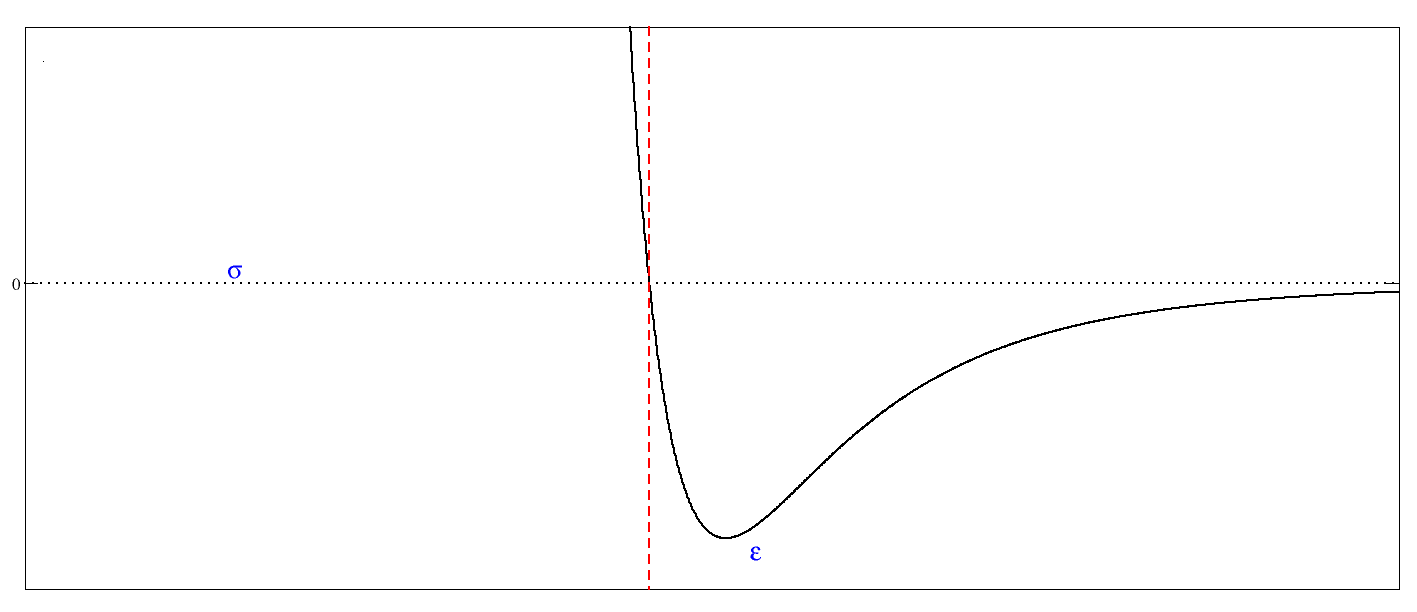
\includegraphics[width=1\textwidth,keepaspectratio=true]{LJ.png}
    \caption{Potencial Lennard-Jones}
    \label{fig:LJ126}
\end{figure}

\newpage

Este potencial esta dividido en tres intervalos en el eje $r$ \cite{ADAMS2001763}:

\begin{itemize}
    \item El primer intervalo es el potencial repulsivo que esta antes de la linea roja en la figura \ref{fig:LJ126}, este es para evitar el traslape de nubes electrónicas (Principio de exclusión de pauli).
    \item El pozo del potencial es debido a la cohesión en la fase condensada de la materia.
    \item La parte atractiva de este potencial es creada por dipolos temporales por fluctuaciones de las nubes electronicas \cite{INOUE2011157}.
\end{itemize}

\begingroup
\let\clearpage\relax
\chapter{Nanotubos de carbono}
\endgroup

\section{Estructura de los nanotubos de carbono}

En la simulación presentada se usó un nanotubo de carbono de una capa (SWCNT por sus siglas en ingles), así, es de interés explicar caracteristicas, geometría y algunas propiedades.\\

\begin{table}[h!]
    \centering
    \begin{tabular}{ |p{2cm}|p{3cm}|  }
    \hline
    \multicolumn{2}{|c|}{Caracteristicas} \\
    \hline
    $a_{cc}$   & 1.42 \AA \\
    \hline
    C-C-C($\theta$)   & 120 $\deg$ \\
    \hline
    q & 0e \\
    \hline
    m   & 12.0107 u \\
    \hline
    \end{tabular}
    \caption{Caracteristicas del carbono y enlaces de carbono \cite{Melendez2016}}
    \label{carbono}
\end{table}

\newpage

Los nanotubos de carbonos son una sabana de un arreglo hexagonal de carbono enrollados en un eje para formar un cilindro, fueron descubiertos por Iijima en experimentos usando el método de arco de descarga en 1991 \cite{Iijima1991}.\\

\section{Geometría y notación (n,m)}

\begin{figure}[!h] 
    \centering
    \begin{minipage}{0.45\textwidth}
    \centering
    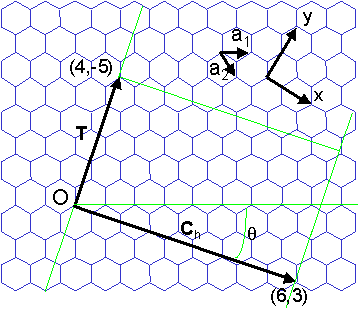
\includegraphics[width=0.95\textwidth]{ChCNT.png}
    \end{minipage}
    \begin{minipage}{0.45\textwidth}
    \centering
    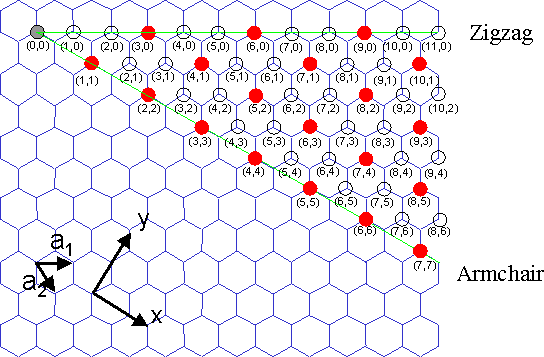
\includegraphics[width=1.2\textwidth]{NT.png}
    \end{minipage}
    \caption{Chiralidad y simetría en nanotubos \cite{ShigeoChiral}}
\end{figure} \label{fig:GeoVectChir}

La geometría se puede describir usando los vectores $\vec{a_1}$ y $\vec{a_2}$ por convención estan arreglados como se muestra en las figuras [2.1]. Usando estos podemos describir las siguientes caracteristicas \cite{Melendez2016}:\\

\begin{itemize}
    \item Vector chiral (n,m): $C_h = n\vec{a_1} + m\vec{a_2}$
    \item Magnitud del vector chiral: $\left|C_h\right| = \sqrt{3}a_{cc}\sqrt{n^2+m^2+nm}$
    \item Diametro del nanotubo: $d_T = \left|C_h\right|/\pi$
\end{itemize}

El vector de traslación $\vec{T}$ es el vector mas corto perpendicular a $C_h$ que empieza y termina en un punto del arreglo hexagonal:

\begin{itemize}
    \item Vector de traslación: $\vec{T} = \left[\left(2m+n\right)\vec{a_1} - \left(2n+m\right)\vec{a_2}\right]/d_R$
    \item Magnitud del vector de traslación: $\left|\vec{T}\right|=\sqrt{3}a_{cc}\frac{\left|C_h\right|}{d_R}$
\end{itemize}

donde:

\begin{equation}\label{dR}
    d_R =
    \begin{cases} 
    d,& \text{si } n-m \text{ no es múltiplo de } 3d\\
    3d,& \text{si } n-m \text{ es múltiplo de } 3d
    \end{cases}
\end{equation}\\

Los nanotubos estan categorizados por su notación (n,m) \cite{Melendez2016}:

\begin{itemize}
    \item Armchair: (n,n) $\left|C_h\right|=3na_{cc}$ y $\left|\vec{T}\right|=\sqrt{3}a_{cc}$
    \item Zigzag: (n,0) $\left|C_h\right|=\sqrt{3}na_{cc}$ y $\left|\vec{T}\right|=3a_{cc}$
    \item Chiral: (n,m) where 0 < m < n
\end{itemize}

Para un SWCNT (n,m), si n = m el nanotubo es metálico; si n - m es múltiplo de 3, el nanotubo es casi-metálico, de otra manera el nanotubo es un semiconductor. En la figura [2.1] los puntos rojos representan los nanotubos metálicos y los círculos negros representan los semiconductores.\\

Lo anterior asegura que la notación (n,m) define completamente la estructura de un SWCNT.

\begingroup
\let\clearpage\relax
\chapter{Dinámica molecular}
\endgroup
